\chapter{Perfect Graphs}
\section{Definition}
\begin{paragraph}
\indent A perfect graph is a graph where the chromatic number of every induced subgraph equals the size of the largest clique of the subgraph.
\end{paragraph}
\section{Example}
\begin{paragraph}
\indent Below is the Paley graph of order nine. As you can see, the chromatic number is 3 and there is one clique of 3 shown with the top three vertices. In each of the subgraphs, the chromatic number equals the clique number, so the graph is a perfect graph.
\end{paragraph}
\newline
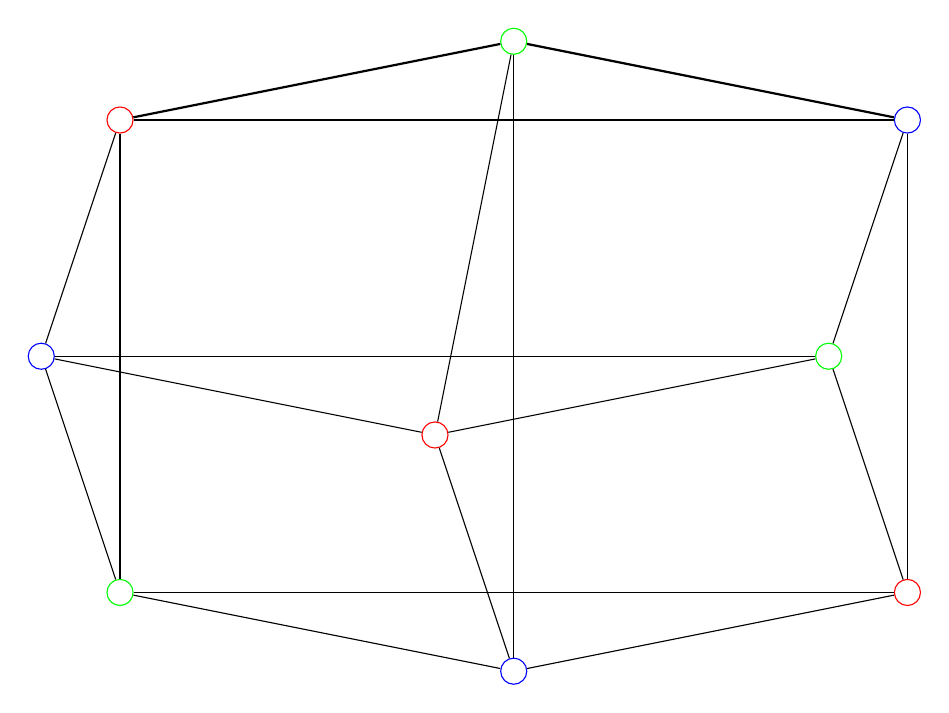
\begin{tikzpicture}
\node[shape=circle,draw=red] (a) at (0,0) {};
\node[shape=circle,draw=green] (b) at (5,1) {};
\node[shape=circle,draw=blue] (c) at (10,0) {};
\node[shape=circle,draw=blue] (d) at (-1,-3) {};
\node[shape=circle,draw=red] (e) at (4,-4) {};
\node[shape=circle,draw=green] (f) at (9,-3) {};
\node[shape=circle,draw=green] (g) at (0,-6) {};
\node[shape=circle,draw=blue] (h) at (5,-7) {};
\node[shape=circle,draw=red] (i) at (10,-6) {};

\draw (a) edge[thick] (b);
\draw (a) edge[thick] (c);
\draw (a)--(d);
\draw (a)--(g);
\draw (b) edge[thick] (c);
\draw (b)--(e);
\draw (b)--(h);
\draw (c)--(f);
\draw (c)--(i);
\draw (d)--(g);
\draw (d)--(e);
\draw (d)--(f);
\draw (e)--(f);
\draw (e)--(h);
\draw (f)--(i);
\draw (g)--(h);
\draw (g)--(i);
\draw (h)--(i);
\end{tikzpicture}

\section{Theorems}
\subsection{Perfect Graph Theorem}
\begin{paragraph}
\indent A graph $G$ is perfect if and only if $\overline{G}$ is perfect.
\end{paragraph}
\subsection{Strong Perfect Graph Theorem}
\begin{paragraph}
\indent A graph $G$ is perfect if an only if neither G nor $\overline{G}$ contains an induced cycle of odd length greater than three.
\end{paragraph}

\section{What Graphs are perfect?}
\begin{paragraph}
\indent There are many graphs that are perfect. Bipartite, chordal, and comparable graphs were mentioned in the notes in class. Others mentioned on the Wikipedia page include line and trapezoid graphs.
\end{paragraph}

\bibliographystyle{plain}
\bibliography{ChapterPerfect/bibliography}
\nocite{*}


